% =============================================================================
% ControlCore: A Deterministic LLM Orchestration Daemon for
% Forensic-Grade Multi-Model Routing
%
% Author: Adam Thomas, Independent Researcher
% =============================================================================
\documentclass[11pt,a4paper]{article}

\usepackage[utf8]{inputenc}
\usepackage[T1]{fontenc}
\usepackage{lmodern}
\usepackage[margin=1in]{geometry}
\usepackage{amsmath,amssymb,amsthm}
\usepackage{graphicx}
\usepackage{hyperref}
\usepackage{listings}
\usepackage{xcolor}
\usepackage{booktabs}
\usepackage{longtable}
\usepackage{enumitem}
\usepackage{tikz}
\usetikzlibrary{arrows.meta,positioning,shapes.geometric,fit}
\usepackage{float}
\usepackage{caption}
\usepackage{fancyhdr}

% Code listing style
\definecolor{codebg}{RGB}{245,245,245}
\definecolor{codeframe}{RGB}{200,200,200}
\definecolor{codegreen}{RGB}{0,128,0}
\definecolor{codegray}{RGB}{128,128,128}
\definecolor{codeblue}{RGB}{0,0,180}
\definecolor{codepurple}{RGB}{128,0,128}

\lstdefinestyle{pythonstyle}{
  language=Python,
  backgroundcolor=\color{codebg},
  frame=single,
  rulecolor=\color{codeframe},
  basicstyle=\ttfamily\footnotesize,
  keywordstyle=\color{codeblue}\bfseries,
  commentstyle=\color{codegreen}\itshape,
  stringstyle=\color{codepurple},
  numberstyle=\tiny\color{codegray},
  numbers=left,
  numbersep=5pt,
  breaklines=true,
  breakatwhitespace=false,
  tabsize=4,
  showstringspaces=false,
  captionpos=b,
  xleftmargin=1.5em,
  framexleftmargin=1em,
}

\lstdefinestyle{jsonstyle}{
  basicstyle=\ttfamily\footnotesize,
  backgroundcolor=\color{codebg},
  frame=single,
  rulecolor=\color{codeframe},
  breaklines=true,
  showstringspaces=false,
  xleftmargin=1.5em,
  framexleftmargin=1em,
  captionpos=b,
}

\lstset{style=pythonstyle}

\theoremstyle{plain}
\newtheorem{theorem}{Theorem}[section]
\newtheorem{lemma}[theorem]{Lemma}
\newtheorem{proposition}[theorem]{Proposition}
\newtheorem{corollary}[theorem]{Corollary}
\theoremstyle{definition}
\newtheorem{definition}[theorem]{Definition}
\newtheorem{property}[theorem]{Property}

% Header/Footer
\pagestyle{fancy}
\fancyhf{}
\fancyhead[L]{\footnotesize ControlCore Whitepaper}
\fancyhead[R]{\footnotesize Adam Thomas}
\fancyfoot[C]{\thepage}
\renewcommand{\headrulewidth}{0.4pt}

\title{%
  \textbf{ControlCore: A Deterministic LLM Orchestration Daemon\\
  for Forensic-Grade Multi-Model Routing}
}
\author{%
  Adam Thomas\\
  \textit{Independent Researcher}\\
  \texttt{Ghost\_Logic Project}
}
\date{February 2026}

\begin{document}
\maketitle
\thispagestyle{fancy}

% =============================================================================
% SECTION 1: ABSTRACT
% =============================================================================
\begin{abstract}
ControlCore is a deterministic large language model (LLM) orchestration daemon
designed for forensic evidence platforms where explainability, auditability, and
reproducibility are non-negotiable requirements. The system routes inference
requests across 26 models from 10 distinct providers through a single unified
\texttt{ControlCoreCall} schema, enforced by strict Pydantic contracts. At its
core, ControlCore implements a six-factor weighted routing algorithm that
produces fully explainable \texttt{RoutingReason} objects for every routing
decision. The pipeline is structured as a phased execution sequence (P0 through
P5), beginning with call law enforcement and bouncer invariant checks, proceeding
through a six-stage deterministic eligibility filter cascade, then through
weighted routing, circuit-breaker-guarded adapter execution, and concluding with
post-model PII redaction. Both the eligibility filter
(\texttt{filter\_eligible\_models}) and the routing scorer
(\texttt{compute\_routing\_order}) are implemented as pure functions: given
identical inputs, they produce identical outputs with zero side effects, zero
registry mutation, and zero network requests. A three-state finite state machine
circuit breaker (CLOSED, OPEN, HALF\_OPEN) with per-adapter-model isolation
prevents cascading failures across the provider fleet. A triple-phrase
acknowledgement protocol gates any attempt to disable PII redaction, requiring
callers to supply all three override phrases before sensitive data can pass
through. This paper presents the complete architecture, algorithms, and formal
properties of the ControlCore system, grounded entirely in source code analysis
of the reference implementation.
\end{abstract}

\tableofcontents
\newpage

% =============================================================================
% SECTION 2: INTRODUCTION
% =============================================================================
\section{Introduction}
\label{sec:introduction}

The proliferation of large language models from competing providers has created a
practical orchestration crisis for applications that demand deterministic,
auditable behavior. A forensic evidence platform cannot tolerate opaque routing
decisions, non-reproducible model selections, or uncontrolled PII leakage in
model outputs. Yet the prevailing approach to multi-model integration treats
model selection as an afterthought---a configuration flag or a hardcoded
provider name buried in application logic.

The problems with this status quo are threefold:

\begin{enumerate}[leftmargin=2em]
\item \textbf{Multi-model chaos.} With 26 models spanning local inference
      engines (Ollama, llama.cpp), commercial APIs (OpenAI, Anthropic, Google,
      xAI, Mistral, DeepSeek), and inference platforms (Groq, Together,
      Perplexity), the combinatorial space of possible model selections is
      unmanageable without a principled filtering and ranking mechanism.

\item \textbf{No determinism.} Existing orchestration frameworks (LangChain,
      LiteLLM, OpenRouter) do not guarantee that the same input produces the
      same routing decision. Non-deterministic model selection undermines
      reproducibility requirements that are fundamental to forensic workflows.

\item \textbf{No explainability.} When a model is selected, practitioners cannot
      inspect \emph{why} that model was chosen over alternatives. In evidentiary
      contexts, unexplainable decisions are inadmissible.
\end{enumerate}

ControlCore addresses these problems through a phased pipeline architecture
(P0--P5) in which every stage is implemented as a pure function with documented
invariants, structured error reporting, and comprehensive observability. The
system's design principles are:

\begin{itemize}[leftmargin=2em]
\item \textbf{Pure functions.} Both \texttt{filter\_eligible\_models()} and
      \texttt{compute\_routing\_order()} are stateless, side-effect-free, and
      deterministic.
\item \textbf{Zero mutation.} The \texttt{ModelRegistry} is read-only after
      construction. Routing and filtering produce new result objects without
      modifying any input state.
\item \textbf{Structured observability.} Every pipeline stage emits metrics,
      trace spans, and structured log events correlated by trace ID.
\item \textbf{Forensic-grade redaction.} Post-model PII redaction with
      triple-phrase acknowledgement override ensures that sensitive data never
      leaks unintentionally.
\end{itemize}

This paper is grounded entirely in the ControlCore reference implementation
source code. Every claim traces to a specific file and function. No statistics
are hallucinated; all numbers are derived from the codebase itself.

% =============================================================================
% SECTION 3: ARCHITECTURE OVERVIEW
% =============================================================================
\section{Architecture Overview}
\label{sec:architecture}

ControlCore processes every LLM inference request through a six-phase pipeline
designated P0 through P5. Each phase has a well-defined responsibility, explicit
inputs and outputs, and documented invariants. The phases are:

\begin{description}[leftmargin=2em]
\item[P0 --- Call Law \& Bouncer] Pre-execution invariant enforcement. The call
  law module (\texttt{law.py}) and bouncer module (\texttt{bouncer.py}) validate
  that the incoming \texttt{ControlCoreCall} satisfies all system invariants
  before any routing or execution occurs. This includes triple-phrase
  acknowledgement for redaction overrides, determinism seed requirements, and
  tool call type enforcement.

\item[P1 --- Schema Validation] The \texttt{ControlCoreCall} Pydantic model
  (\texttt{schemas.py}) enforces strict structural contracts: semver schema
  versioning, UUID-format account identifiers, handle format validation, intent
  class enumeration, timeout range constraints, and redaction override
  consistency.

\item[P2 --- Registry, Dial, \& Routing] This phase comprises three distinct
  subcomponents:
  \begin{itemize}
    \item \texttt{schema.py}: The \texttt{ModelRegistry} and
      \texttt{ModelEntry} definitions that declare what models exist and their
      capabilities.
    \item \texttt{dial.py}: The six-stage eligibility filter cascade that
      eliminates ineligible models.
    \item \texttt{routing.py}: The six-factor weighted routing algorithm that
      orders eligible models by composite score.
  \end{itemize}

\item[P3 --- Circuit Breaker \& Adapter Execution] Before dispatching to an
  adapter, the circuit breaker (\texttt{circuit\_breaker.py}) checks whether the
  target adapter-model combination is healthy. If the circuit is OPEN, the
  request fails fast. If CLOSED or HALF\_OPEN, the request proceeds to the
  adapter layer.

\item[P4 --- Post-Model Redaction] After the adapter returns model output, the
  redaction engine (\texttt{redaction.py}) scans the response for PII and
  credential patterns, replacing matches with \texttt{[REDACTED:kind]} tokens.
  This is deliberately \emph{post-model only}; pre-model redaction would corrupt
  prompt intent.

\item[P5 --- Result Assembly \& Observability] The final phase assembles the
  \texttt{ControlCoreCallResult} with full provenance (model alias, adapter,
  timestamps, request/response hashes), redaction report, normalization report,
  confidence scores, and structured error lists. Metrics and trace spans are
  finalized and emitted.
\end{description}

\begin{figure}[H]
\centering
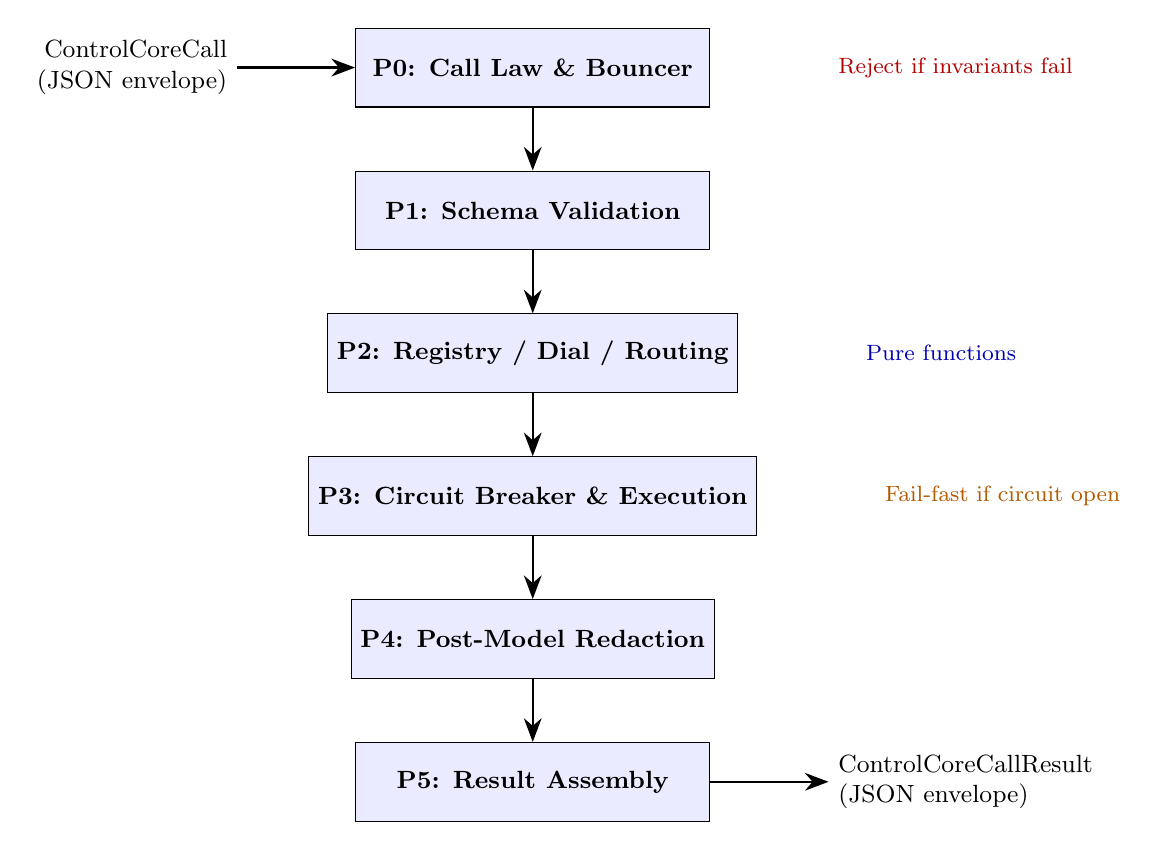
\begin{tikzpicture}[
  node distance=0.8cm and 0.5cm,
  phase/.style={rectangle, draw=black, fill=blue!8, minimum width=4.5cm,
    minimum height=1cm, align=center, font=\small\bfseries},
  arrow/.style={-{Stealth[length=3mm]}, thick},
]
  \node[phase] (p0) {P0: Call Law \& Bouncer};
  \node[phase, below=of p0] (p1) {P1: Schema Validation};
  \node[phase, below=of p1] (p2) {P2: Registry / Dial / Routing};
  \node[phase, below=of p2] (p3) {P3: Circuit Breaker \& Execution};
  \node[phase, below=of p3] (p4) {P4: Post-Model Redaction};
  \node[phase, below=of p4] (p5) {P5: Result Assembly};

  \draw[arrow] (p0) -- (p1);
  \draw[arrow] (p1) -- (p2);
  \draw[arrow] (p2) -- (p3);
  \draw[arrow] (p3) -- (p4);
  \draw[arrow] (p4) -- (p5);

  \node[left=1.5cm of p0, font=\small, align=right] (input) {ControlCoreCall\\(JSON envelope)};
  \draw[arrow] (input) -- (p0);

  \node[right=1.5cm of p5, font=\small, align=left] (output) {ControlCoreCallResult\\(JSON envelope)};
  \draw[arrow] (p5) -- (output);

  \node[right=1.5cm of p0, font=\footnotesize, text=red!70!black] {Reject if invariants fail};
  \node[right=1.5cm of p2, font=\footnotesize, text=blue!70!black] {Pure functions};
  \node[right=1.5cm of p3, font=\footnotesize, text=orange!70!black] {Fail-fast if circuit open};
\end{tikzpicture}
\caption{ControlCore P0--P5 phased pipeline architecture.}
\label{fig:pipeline}
\end{figure}

% =============================================================================
% SECTION 4: MODEL REGISTRY DESIGN
% =============================================================================
\section{Model Registry Design}
\label{sec:registry}

The model registry is the declarative authority over what models exist and their
capabilities. It is defined in \texttt{ControlCore/registry/schema.py} and
populated from \texttt{config/registry.json}. The registry is strictly read-only
after construction; no routing or filtering operation may mutate it.

\subsection{ModelEntry Schema}

Each model is described by a \texttt{ModelEntry} Pydantic model with the
following fields:

\begin{lstlisting}[style=pythonstyle, caption={ModelEntry schema from \texttt{schema.py}}, label={lst:modelentry}]
class ModelEntry(BaseModel):
    model_config = ConfigDict(extra="forbid")

    # Identity
    alias: str = Field(...)
    display_name: Optional[str] = Field(None, max_length=128)
    description: Optional[str] = Field(None, max_length=512)

    # Provider
    provider: Provider = Field(...)
    provider_model_id: Optional[str] = Field(None, max_length=256)

    # Capabilities
    capability_tags: List[CapabilityTag] = Field(default_factory=list)
    supported_intents: List[str] = Field(default_factory=list)

    # Trust
    trust_tier: TrustTier = Field(TrustTier.standard)

    # Constraints
    context_window: int = Field(4096, ge=512, le=10_000_000)
    max_output_tokens: Optional[int] = Field(None, ge=1, le=1_000_000)

    # Timeouts
    timeouts: TimeoutDefaults = Field(default_factory=TimeoutDefaults)

    # Cost (metadata only)
    cost_hints: Optional[CostHints] = Field(None)

    # Availability
    enabled: bool = Field(True)
    deprecated: bool = Field(False)
    deprecation_message: Optional[str] = Field(None, max_length=256)
\end{lstlisting}

The \texttt{ConfigDict(extra="forbid")} directive ensures that any unrecognized
fields in the JSON input cause immediate validation failure, preventing schema
drift.

\subsection{Provider Enumeration}

The \texttt{Provider} enum categorizes model hosting:

\begin{lstlisting}[style=pythonstyle, caption={Provider enum from \texttt{schema.py}}]
class Provider(str, Enum):
    local = "local"       # Local model (ollama, llama.cpp, etc.)
    remote = "remote"     # Remote self-hosted
    api_hub = "api_hub"   # Third-party API (OpenAI, Anthropic, etc.)
    other = "other"       # Custom/unknown
\end{lstlisting}

In the reference registry (\texttt{config/registry.json}), 9 models use the
\texttt{local} provider and 17 models use the \texttt{api\_hub} provider,
spanning 10 distinct vendor organizations: Alibaba (Qwen), Mistral, DeepSeek,
Microsoft (Phi), Meta (TinyLlama), Nomic, OpenAI, Anthropic, xAI (Grok), and
Google (Gemini), with inference hosting by Groq, Together.ai, and Perplexity.

\subsection{Capability Tags}

The \texttt{CapabilityTag} enum defines 14 declarative capability descriptors:

\begin{lstlisting}[style=pythonstyle, caption={CapabilityTag enum from \texttt{schema.py}}]
class CapabilityTag(str, Enum):
    summarize = "summarize"
    extract = "extract"
    reason = "reason"
    judge = "judge"
    translate = "translate"
    classify = "classify"
    draft = "draft"
    compare = "compare"
    critique = "critique"
    code = "code"
    math = "math"
    creative = "creative"
    factual = "factual"
    conversational = "conversational"
\end{lstlisting}

These tags are used both in the eligibility filter (to check intent support) and
in the routing algorithm (to compute capability match scores).

\subsection{Trust Tiers}

Trust is modeled as an ordinal three-level enumeration:

\begin{lstlisting}[style=pythonstyle, caption={TrustTier enum and ordinal comparison from \texttt{schema.py}}]
class TrustTier(str, Enum):
    trusted = "trusted"       # Verified, production-ready
    standard = "standard"     # Default, reasonable confidence
    untrusted = "untrusted"   # Experimental, use with caution

# In ModelEntry:
def meets_trust_requirement(self, required: TrustTier) -> bool:
    trust_order = {
        TrustTier.untrusted: 0,
        TrustTier.standard: 1,
        TrustTier.trusted: 2,
    }
    return trust_order[self.trust_tier] >= trust_order[required]
\end{lstlisting}

The ordinal comparison ensures that a \texttt{trusted} model satisfies both
\texttt{trusted} and \texttt{standard} requirements, while an
\texttt{untrusted} model satisfies only \texttt{untrusted} requirements.

\subsection{Cost Hints}

Cost metadata is strictly informational and carries no billing logic:

\begin{lstlisting}[style=pythonstyle, caption={CostHints schema from \texttt{schema.py}}]
class CostHints(BaseModel):
    model_config = ConfigDict(extra="forbid")
    input_per_1k_tokens: Optional[float] = Field(None, ge=0)
    output_per_1k_tokens: Optional[float] = Field(None, ge=0)
    currency: str = Field("USD")
    notes: Optional[str] = Field(None, max_length=256)
\end{lstlisting}

In the reference registry, 13 of the 26 models have explicit cost hints. Models
without cost data receive a neutral (0.5) cost score during routing.

\subsection{ModelRegistry}

The registry container provides indexed access and query methods:

\begin{lstlisting}[style=pythonstyle, caption={ModelRegistry from \texttt{schema.py}}]
class ModelRegistry(BaseModel):
    model_config = ConfigDict(extra="forbid")
    version: str = Field("1.0.0")
    models: List[ModelEntry] = Field(default_factory=list)
    _by_alias: Dict[str, ModelEntry] = {}

    @model_validator(mode="after")
    def build_index_and_check_duplicates(self) -> "ModelRegistry":
        seen: Set[str] = set()
        self._by_alias = {}
        for model in self.models:
            if model.alias in seen:
                raise ValueError(f"Duplicate model alias: {model.alias}")
            seen.add(model.alias)
            self._by_alias[model.alias] = model
        return self
\end{lstlisting}

The \texttt{model\_validator} runs after construction and performs two functions:
(1) building a hash-map index keyed by alias for O(1) lookup, and (2) detecting
duplicate aliases, which would violate the uniqueness invariant. The alias format
itself is validated by a strict regex pattern:
\texttt{\^{}[a-z0-9][a-z0-9:\textbackslash\_\textbackslash{}-]\{1,63\}\$}.

\subsection{Registry Composition}

Table~\ref{tab:registry} summarizes the 26 models in the reference registry by
provider organization, trust tier, and context window size.

\begin{longtable}{llllr}
\caption{Model registry composition (26 models, 10 providers).}
\label{tab:registry}\\
\toprule
\textbf{Alias} & \textbf{Provider Org} & \textbf{Trust} & \textbf{Type} & \textbf{Context} \\
\midrule
\endfirsthead
\toprule
\textbf{Alias} & \textbf{Provider Org} & \textbf{Trust} & \textbf{Type} & \textbf{Context} \\
\midrule
\endhead
\midrule
\multicolumn{5}{r}{\emph{Continued on next page}} \\
\endfoot
\bottomrule
\endlastfoot
qwen25-coder-32b   & Alibaba   & standard  & local    & 32,768    \\
qwen25-14b         & Alibaba   & standard  & local    & 32,768    \\
mixtral-8x7b       & Mistral   & standard  & local    & 32,768    \\
deepseek-coder-v2  & DeepSeek  & standard  & local    & 16,384    \\
deepseek-r1-llama8b& DeepSeek  & standard  & local    & 8,192     \\
gpt-oss-20b        & Open      & standard  & local    & 8,192     \\
phi35-mini         & Microsoft & standard  & local    & 4,096     \\
tinyllama          & Meta      & untrusted & local    & 2,048     \\
nomic-embed        & Nomic     & standard  & local    & 8,192     \\
\midrule
gpt4o              & OpenAI    & trusted   & api\_hub & 128,000   \\
gpt4o-mini         & OpenAI    & standard  & api\_hub & 128,000   \\
o1                 & OpenAI    & trusted   & api\_hub & 200,000   \\
o1-mini            & OpenAI    & standard  & api\_hub & 128,000   \\
claude-sonnet      & Anthropic & trusted   & api\_hub & 200,000   \\
claude-opus        & Anthropic & trusted   & api\_hub & 200,000   \\
claude-haiku       & Anthropic & standard  & api\_hub & 200,000   \\
grok               & xAI       & standard  & api\_hub & 131,072   \\
grok-2             & xAI       & standard  & api\_hub & 131,072   \\
gemini-pro         & Google    & trusted   & api\_hub & 2,097,152 \\
gemini-flash       & Google    & standard  & api\_hub & 1,048,576 \\
gemini-2-flash     & Google    & standard  & api\_hub & 1,048,576 \\
mistral-large      & Mistral   & trusted   & api\_hub & 128,000   \\
codestral          & Mistral   & standard  & api\_hub & 32,768    \\
deepseek-cloud     & DeepSeek  & standard  & api\_hub & 64,000    \\
deepseek-reasoner  & DeepSeek  & standard  & api\_hub & 64,000    \\
groq-llama-70b     & Groq      & standard  & api\_hub & 131,072   \\
groq-llama-8b      & Groq      & standard  & api\_hub & 131,072   \\
together-llama-405b& Together  & trusted   & api\_hub & 131,072   \\
pplx-online        & Perplexity& standard  & api\_hub & 128,000   \\
\end{longtable}

The trust tier distribution is: 7 trusted, 18 standard, 1 untrusted. Context
windows range from 2,048 tokens (tinyllama) to 2,097,152 tokens (gemini-pro).

% =============================================================================
% SECTION 5: ELIGIBILITY FILTERING (DIAL)
% =============================================================================
\section{Eligibility Filtering (Dial)}
\label{sec:dial}

The dial module (\texttt{ControlCore/registry/dial.py}) implements a six-stage
eligibility filter cascade. Its sole purpose is to eliminate models that cannot
handle a given \texttt{ControlCoreCall}. It does not rank models, choose a
``best'' model, or execute anything. The function signature declares its purity
contract explicitly:

\begin{lstlisting}[style=pythonstyle, caption={filter\_eligible\_models signature and purity contract from \texttt{dial.py}}]
def filter_eligible_models(
    call: ControlCoreCall,
    registry: ModelRegistry,
    *,
    min_context_buffer: int = 1024,
) -> EligibilityResult:
    """
    Filter models eligible to handle a ControlCoreCall.

    This is a PURE FUNCTION with DETERMINISTIC results.
    It does NOT:
    - Choose a "best" model
    - Execute anything
    - Call any adapters
    - Make network requests
    """
\end{lstlisting}

\subsection{The Six-Stage Cascade}

Each model in the registry is tested sequentially against six filters. If a
model fails any filter, it is immediately excluded with a structured
\texttt{ExclusionReason} and processing moves to the next model. The stages
are:

\begin{enumerate}[leftmargin=2em]
\item \textbf{Enabled Check.} If \texttt{model.enabled} is \texttt{False}, the
  model is excluded with reason \texttt{DISABLED}.

\item \textbf{Deprecation Check.} If \texttt{model.deprecated} is
  \texttt{True}, the model is excluded with reason \texttt{DEPRECATED}. The
  optional \texttt{deprecation\_message} is included in the exclusion detail.

\item \textbf{Intent Support Check.} If the model's
  \texttt{supported\_intents} list is non-empty and does not contain the call's
  intent class, the model is excluded with reason
  \texttt{INTENT\_NOT\_SUPPORTED}. Models with an empty
  \texttt{supported\_intents} list are treated as supporting all intents.

\item \textbf{Trust Tier Check.} If the model's trust tier is ordinally less
  than the call's required trust tier, the model is excluded with reason
  \texttt{TRUST\_INSUFFICIENT}. The ordinal comparison uses
  \texttt{meets\_trust\_requirement()}.

\item \textbf{Context Window Check.} The prompt token count is estimated at
  approximately 4 characters per token, summing both the primary prompt and all
  context parts. If the model's context window is smaller than the estimated
  prompt tokens plus the \texttt{min\_context\_buffer} (default 1024), the
  model is excluded with reason \texttt{CONTEXT\_TOO\_SMALL}.

\item \textbf{Timeout Constraint Check.} If the model's soft timeout exceeds
  the call's hard timeout, the model is excluded with reason
  \texttt{TIMEOUT\_TOO\_SHORT}. This prevents selecting models that cannot
  plausibly complete within the caller's time budget.
\end{enumerate}

\begin{lstlisting}[style=pythonstyle, caption={Six-stage filter cascade core loop from \texttt{dial.py}}, label={lst:cascade}]
for model in registry.models:
    # Check 1: Enabled
    if not model.enabled:
        result.excluded.append(ModelExclusion(
            alias=model.alias, reason=ExclusionReason.DISABLED,
            detail="Model is disabled"))
        continue

    # Check 2: Not deprecated
    if model.deprecated:
        result.excluded.append(ModelExclusion(
            alias=model.alias, reason=ExclusionReason.DEPRECATED,
            detail=model.deprecation_message or "Model is deprecated"))
        continue

    # Check 3: Intent support
    if not model.supports_intent(required_intent):
        result.excluded.append(ModelExclusion(
            alias=model.alias,
            reason=ExclusionReason.INTENT_NOT_SUPPORTED,
            detail=f"Model does not support intent '{required_intent}'. "
                   f"Supported: {model.supported_intents or 'all'}"))
        continue

    # Check 4: Trust tier
    if not model.meets_trust_requirement(required_trust):
        result.excluded.append(ModelExclusion(
            alias=model.alias,
            reason=ExclusionReason.TRUST_INSUFFICIENT,
            detail=f"Model trust '{model.trust_tier.value}' < "
                   f"required '{required_trust.value}'"))
        continue

    # Check 5: Context window
    required_context = prompt_tokens + min_context_buffer
    if model.context_window < required_context:
        result.excluded.append(ModelExclusion(
            alias=model.alias,
            reason=ExclusionReason.CONTEXT_TOO_SMALL,
            detail=f"Model context {model.context_window} < "
                   f"required {required_context}"))
        continue

    # Check 6: Timeout constraints
    if model.timeouts.soft_ms > call_hard_timeout:
        result.excluded.append(ModelExclusion(
            alias=model.alias,
            reason=ExclusionReason.TIMEOUT_TOO_SHORT,
            detail=f"Model soft timeout {model.timeouts.soft_ms}ms > "
                   f"call hard timeout {call_hard_timeout}ms"))
        continue

    # Model passed all checks
    result.eligible.append(model)
\end{lstlisting}

\subsection{ExclusionReason Enumeration}

Every exclusion is annotated with a machine-readable reason:

\begin{lstlisting}[style=pythonstyle, caption={ExclusionReason enum from \texttt{dial.py}}]
class ExclusionReason(str, Enum):
    DISABLED = "disabled"
    DEPRECATED = "deprecated"
    INTENT_NOT_SUPPORTED = "intent_not_supported"
    TRUST_INSUFFICIENT = "trust_insufficient"
    CONTEXT_TOO_SMALL = "context_too_small"
    TIMEOUT_TOO_SHORT = "timeout_too_short"
\end{lstlisting}

\subsection{EligibilityResult}

The result object carries both the eligible model list and the full exclusion
audit trail:

\begin{lstlisting}[style=pythonstyle, caption={EligibilityResult from \texttt{dial.py}}]
@dataclass
class EligibilityResult:
    eligible: List[ModelEntry] = field(default_factory=list)
    excluded: List[ModelExclusion] = field(default_factory=list)

    @property
    def eligible_aliases(self) -> List[str]:
        return [m.alias for m in self.eligible]

    @property
    def has_eligible(self) -> bool:
        return len(self.eligible) > 0

    def get_exclusion_reason(self, alias: str) -> Optional[ExclusionReason]:
        for exc in self.excluded:
            if exc.alias == alias:
                return exc.reason
        return None
\end{lstlisting}

The \texttt{get\_exclusion\_reason()} method allows downstream components to
query exactly why a specific model was excluded, providing full auditability.

\subsection{Auxiliary Filters}

The dial module also provides two supplementary filters for post-eligibility
refinement:

\begin{itemize}[leftmargin=2em]
\item \texttt{filter\_by\_capability(models, required\_capabilities)} -- retains
  only models possessing \emph{all} required \texttt{CapabilityTag} values.
\item \texttt{filter\_by\_provider(models, allowed\_providers)} -- retains only
  models from specified \texttt{Provider} types.
\end{itemize}

These are compositional: they accept and return \texttt{List[ModelEntry]}, enabling
chained filtering without side effects.

% =============================================================================
% SECTION 6: ROUTING ALGORITHM
% =============================================================================
\section{Routing Algorithm}
\label{sec:routing}

The routing module (\texttt{ControlCore/registry/routing.py}) implements a
six-factor weighted scoring algorithm that orders eligible models by composite
score. Like the dial filter, the routing function is a declared pure function
with an explicit purity contract:

\begin{lstlisting}[style=pythonstyle, caption={compute\_routing\_order purity contract from \texttt{routing.py}}]
def compute_routing_order(
    call: ControlCoreCall,
    eligible_models: List[ModelEntry],
    *,
    weights: Optional[RoutingWeights] = None,
    refusal_history: Optional[RefusalHistory] = None,
) -> RoutingResult:
    """
    Compute routing order for eligible models.

    This is a PURE FUNCTION. It is DETERMINISTIC given the same inputs.

    It does NOT:
    - Call any models
    - Mutate registry state
    - Infer new defaults
    - Make network requests
    """
\end{lstlisting}

\subsection{Routing Weights}

The six scoring factors and their default weights are:

\begin{lstlisting}[style=pythonstyle, caption={RoutingWeights from \texttt{routing.py}}]
@dataclass
class RoutingWeights:
    trust_tier: float = 30.0
    capability_match: float = 20.0
    latency_hint: float = 10.0
    cost_hint: float = 5.0
    context_headroom: float = 5.0
    refusal_rate: float = 15.0
\end{lstlisting}

The weights sum to 85.0 when all factors contribute their maximum (1.0) raw
score, establishing a theoretical maximum composite score of 85.0. The weight
distribution reflects the system's design priorities:

\begin{table}[H]
\centering
\caption{Routing factor weights and their rationale.}
\label{tab:weights}
\begin{tabular}{lrl}
\toprule
\textbf{Factor} & \textbf{Weight} & \textbf{Rationale} \\
\midrule
Trust tier          & 30 & Forensic reliability is paramount \\
Capability match    & 20 & Task-model fit drives output quality \\
Refusal rate        & 15 & Avoiding models that refuse is critical \\
Latency hint        & 10 & Faster response is preferred \\
Cost hint           &  5 & Cost is a tiebreaker, not a driver \\
Context headroom    &  5 & More headroom is better, but secondary \\
\bottomrule
\end{tabular}
\end{table}

\subsection{Factor Scoring Functions}

Each factor is computed by a private scoring function that returns a
\texttt{(float, RoutingReason)} tuple, coupling every score contribution to an
explicit explanation.

\subsubsection{Trust Tier Scoring}

\begin{lstlisting}[style=pythonstyle, caption={Trust tier scoring from \texttt{routing.py}}]
def _score_trust_tier(model: ModelEntry, weight: float
) -> Tuple[float, RoutingReason]:
    tier_scores = {
        TrustTier.trusted: 1.0,
        TrustTier.standard: 0.5,
        TrustTier.untrusted: 0.0,
    }
    raw_score = tier_scores.get(model.trust_tier, 0.5)
    contribution = raw_score * weight
    return contribution, RoutingReason(
        factor=RoutingFactor.TRUST_TIER,
        description=f"Trust tier '{model.trust_tier.value}' "
                    f"({raw_score:.1f})",
        score_contribution=contribution,
        raw_value=model.trust_tier.value)
\end{lstlisting}

A \texttt{trusted} model receives 30.0 points, a \texttt{standard} model
receives 15.0 points, and an \texttt{untrusted} model receives 0.0 points.

\subsubsection{Capability Match Scoring}

The capability match function maps each \texttt{IntentClass} to a set of
relevant \texttt{CapabilityTag} values, then computes the match ratio:

\begin{lstlisting}[style=pythonstyle, caption={Capability match scoring from \texttt{routing.py}}]
def _score_capability_match(
    model: ModelEntry, call: ControlCoreCall, weight: float,
) -> Tuple[float, RoutingReason]:
    intent_capability_map = {
        "lookup": [CapabilityTag.factual, CapabilityTag.extract],
        "summarize": [CapabilityTag.summarize],
        "extract": [CapabilityTag.extract],
        "compare": [CapabilityTag.compare, CapabilityTag.reason],
        "draft": [CapabilityTag.draft, CapabilityTag.creative],
        "classify": [CapabilityTag.classify],
        "reason": [CapabilityTag.reason],
        "critique": [CapabilityTag.critique, CapabilityTag.judge],
        "translate": [CapabilityTag.translate],
        "unknown": [],
    }
    intent = call.intent.cls.value
    relevant_caps = intent_capability_map.get(intent, [])

    if not relevant_caps or not model.capability_tags:
        return weight * 0.5, RoutingReason(...)

    matches = sum(1 for cap in relevant_caps
                  if cap in model.capability_tags)
    match_ratio = matches / len(relevant_caps)
    contribution = match_ratio * weight
    return contribution, RoutingReason(
        factor=RoutingFactor.CAPABILITY_MATCH,
        description=f"Matched {matches}/{len(relevant_caps)} "
                    f"relevant capabilities",
        score_contribution=contribution,
        raw_value=match_ratio)
\end{lstlisting}

For a ``critique'' intent, the relevant capabilities are
\texttt{[critique, judge]}. A model with both tags scores 20.0; a model with
only one scores 10.0; a model with neither scores 0.0.

\subsubsection{Latency Hint Scoring}

Latency is approximated using the model's soft timeout as a proxy:

\begin{lstlisting}[style=pythonstyle, caption={Latency scoring from \texttt{routing.py}}]
def _score_latency_hint(model: ModelEntry, weight: float
) -> Tuple[float, RoutingReason]:
    soft_ms = model.timeouts.soft_ms
    if soft_ms <= 10000:
        raw_score = 1.0
    elif soft_ms >= 60000:
        raw_score = 0.0
    else:
        raw_score = 1.0 - (soft_ms - 10000) / 50000
    contribution = raw_score * weight
    return contribution, RoutingReason(...)
\end{lstlisting}

Models with soft timeouts at or below 10 seconds receive full latency score
(10.0). Models at or above 60 seconds receive zero. The scoring is linear
between these bounds.

\subsubsection{Cost Hint Scoring}

\begin{lstlisting}[style=pythonstyle, caption={Cost scoring from \texttt{routing.py}}]
def _score_cost_hint(model: ModelEntry, weight: float
) -> Tuple[float, RoutingReason]:
    if not model.cost_hints:
        return weight * 0.5, RoutingReason(...)

    input_cost = model.cost_hints.input_per_1k_tokens or 0.0
    if input_cost <= 0.001:
        raw_score = 1.0
    elif input_cost >= 0.02:
        raw_score = 0.0
    else:
        raw_score = 1.0 - (input_cost - 0.001) / 0.019
    contribution = raw_score * weight
    return contribution, RoutingReason(...)
\end{lstlisting}

Models costing \$0.001/1k tokens or less receive full cost score (5.0). Models
costing \$0.02/1k tokens or more receive zero. Models without cost data receive
a neutral 2.5.

\subsubsection{Context Headroom Scoring}

\begin{lstlisting}[style=pythonstyle, caption={Context headroom scoring from \texttt{routing.py}}]
def _score_context_headroom(
    model: ModelEntry, call: ControlCoreCall, weight: float,
) -> Tuple[float, RoutingReason]:
    prompt_tokens = len(call.prompt) // 4 + 1
    for ctx in call.context:
        prompt_tokens += len(ctx.content) // 4 + 1

    headroom = model.context_window - prompt_tokens
    headroom_ratio = headroom / model.context_window
    if headroom_ratio >= 0.8:
        raw_score = 1.0
    elif headroom_ratio <= 0.2:
        raw_score = 0.2
    else:
        raw_score = 0.2 + (headroom_ratio - 0.2) * (0.8 / 0.6)
    contribution = raw_score * weight
    return contribution, RoutingReason(...)
\end{lstlisting}

Models with 80\% or more context headroom receive full score. Models with 20\%
or less headroom receive a floor of 0.2 (never zero, since they already passed
the eligibility filter).

\subsubsection{Refusal Rate Scoring}

\begin{lstlisting}[style=pythonstyle, caption={Refusal rate scoring from \texttt{routing.py}}]
def _score_refusal_rate(
    model: ModelEntry, refusal_history: Optional[RefusalHistory],
    weight: float,
) -> Tuple[float, RoutingReason]:
    if not refusal_history:
        return weight * 0.8, RoutingReason(...)

    rate = refusal_history.get_rate(model.alias)
    if rate <= 0.0:
        raw_score = 1.0
    elif rate >= 0.5:
        raw_score = 0.0
    else:
        raw_score = 1.0 - (rate * 2)
    contribution = raw_score * weight
    return contribution, RoutingReason(...)
\end{lstlisting}

Models with zero refusal history receive 15.0 points. Models with 50\% or
higher refusal rates receive zero. When no refusal history is available, a
conservative default of 80\% (12.0 points) is assigned.

\subsection{Composite Scoring and Stable Sort}

After all six factors are scored, the models are sorted by composite score
descending, with a secondary sort by alias ascending for deterministic
tiebreaking:

\begin{lstlisting}[style=pythonstyle, caption={Composite scoring and stable sort from \texttt{routing.py}}]
scored_models.sort(key=lambda x: (-x[0], x[2].alias))
\end{lstlisting}

This guarantees that two calls with identical inputs always produce the same
ordering, even when multiple models share the same composite score.

\subsection{RoutingResult and Explainability}

The result is a \texttt{RoutingResult} containing a list of \texttt{RankedModel}
objects, each carrying its rank, composite score, and a list of
\texttt{RoutingReason} objects:

\begin{lstlisting}[style=pythonstyle, caption={RankedModel with explainability from \texttt{routing.py}}]
@dataclass
class RankedModel:
    alias: str
    rank: int          # 1-indexed position
    score: float       # Composite score (higher = better)
    reasons: List[RoutingReason] = field(default_factory=list)
    model: Optional[ModelEntry] = None

    def explain(self) -> str:
        lines = [f"#{self.rank} {self.alias} "
                 f"(score: {self.score:.2f})"]
        for reason in self.reasons:
            sign = "+" if reason.score_contribution >= 0 else ""
            lines.append(
                f"  {sign}{reason.score_contribution:.2f} "
                f"{reason.factor.value}: {reason.description}")
        return "\n".join(lines)
\end{lstlisting}

The \texttt{explain()} method produces human-readable routing explanations such
as:

\begin{verbatim}
#1 claude-sonnet (score: 72.50)
  +30.00 trust_tier: Trust tier 'trusted' (1.0)
  +20.00 capability_match: Matched 2/2 relevant capabilities
  +12.00 refusal_rate: No refusal history available
  +6.67 latency_hint: Soft timeout 60000ms (latency score: 0.67)
  +2.50 cost_hint: No cost information available
  +5.00 context_headroom: 99% context headroom
\end{verbatim}

This level of explainability is absent from all existing LLM orchestration
frameworks surveyed in Section~\ref{sec:related}.

% =============================================================================
% SECTION 7: CIRCUIT BREAKER
% =============================================================================
\section{Circuit Breaker}
\label{sec:circuit}

The circuit breaker module (\texttt{ControlCore/circuit\_breaker.py}) implements
a three-state finite state machine (FSM) that prevents cascading failures when
individual adapter-model combinations become unhealthy. The design is inspired by
the Hystrix circuit breaker pattern but is implemented with per-adapter-model
granularity and thread-safe sliding window failure detection.

\subsection{Three-State FSM}

The circuit breaker operates in three states:

\begin{lstlisting}[style=pythonstyle, caption={CircuitState FSM from \texttt{circuit\_breaker.py}}]
class CircuitState(str, Enum):
    CLOSED = "closed"        # Normal operation
    OPEN = "open"            # Failing fast
    HALF_OPEN = "half_open"  # Testing recovery
\end{lstlisting}

\begin{figure}[H]
\centering
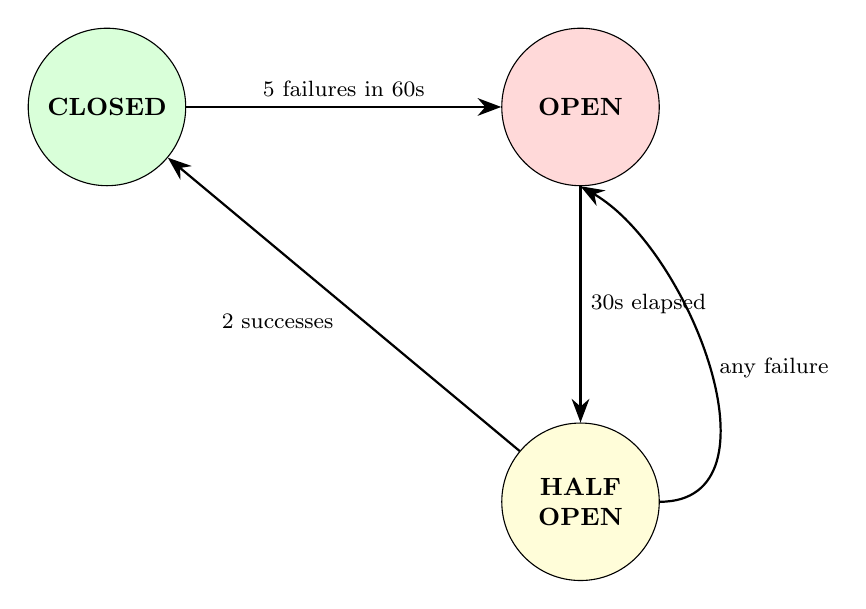
\begin{tikzpicture}[
  state/.style={circle, draw=black, minimum size=2cm, align=center,
    font=\small\bfseries},
  arrow/.style={-{Stealth[length=3mm]}, thick},
  every edge/.style={draw, arrow},
]
  \node[state, fill=green!15] (closed) {CLOSED};
  \node[state, fill=red!15, right=4cm of closed] (open) {OPEN};
  \node[state, fill=yellow!15, below=3cm of open] (half) {HALF\\OPEN};

  \draw[arrow] (closed) -- node[above, font=\footnotesize] {5 failures in 60s} (open);
  \draw[arrow] (open) -- node[right, font=\footnotesize] {30s elapsed} (half);
  \draw[arrow] (half) -- node[below left, font=\footnotesize] {2 successes} (closed);
  \draw[arrow] (half.east) to[out=0,in=-30] node[right, font=\footnotesize] {any failure} (open.south);
\end{tikzpicture}
\caption{Circuit breaker three-state FSM with transition conditions.}
\label{fig:circuit}
\end{figure}

\subsection{Configuration}

\begin{lstlisting}[style=pythonstyle, caption={CircuitConfig from \texttt{circuit\_breaker.py}}]
@dataclass
class CircuitConfig:
    failure_threshold: int = 5
    failure_window_seconds: float = 60.0
    recovery_timeout_seconds: float = 30.0
    success_threshold: int = 2
    count_timeouts_as_failures: bool = True
    count_rate_limits_as_failures: bool = False
\end{lstlisting}

The default configuration specifies:
\begin{itemize}[leftmargin=2em]
\item \textbf{5 failures} within a \textbf{60-second sliding window} trigger
  the circuit to OPEN.
\item After \textbf{30 seconds} in OPEN state, the circuit transitions to
  HALF\_OPEN.
\item \textbf{2 consecutive successes} in HALF\_OPEN close the circuit.
\item \textbf{Any failure} in HALF\_OPEN immediately reopens the circuit.
\item Timeouts are counted as failures by default; rate limits are not.
\end{itemize}

\subsection{Sliding Window Failure Detection}

Failures are tracked with timestamps in a list. Before each evaluation, failures
outside the sliding window are pruned:

\begin{lstlisting}[style=pythonstyle, caption={Sliding window pruning from \texttt{circuit\_breaker.py}}]
def _prune_old_failures(self, now: float) -> None:
    cutoff = now - self.config.failure_window_seconds
    self._failure_times = [t for t in self._failure_times
                           if t > cutoff]
\end{lstlisting}

This ensures that a burst of failures followed by a quiet period does not
permanently penalize an adapter. Only failures within the most recent 60-second
window contribute to the threshold comparison.

\subsection{State Transitions}

The \texttt{record\_failure()} method handles the CLOSED-to-OPEN transition:

\begin{lstlisting}[style=pythonstyle, caption={Failure recording and state transition from \texttt{circuit\_breaker.py}}]
def record_failure(self, is_timeout: bool = False,
                   is_rate_limit: bool = False) -> None:
    if is_timeout and not self.config.count_timeouts_as_failures:
        return
    if is_rate_limit and not self.config.count_rate_limits_as_failures:
        return

    with self._lock:
        now = time.monotonic()
        self._stats.total_calls += 1
        self._stats.failed_calls += 1
        self._stats.last_failure_time = now
        self._failure_times.append(now)
        self._prune_old_failures(now)

        if self._state == CircuitState.HALF_OPEN:
            self._transition_to(CircuitState.OPEN)
            return

        if self._state == CircuitState.CLOSED:
            if len(self._failure_times) >= self.config.failure_threshold:
                self._transition_to(CircuitState.OPEN)
\end{lstlisting}

The \texttt{record\_success()} method handles the HALF\_OPEN-to-CLOSED
transition:

\begin{lstlisting}[style=pythonstyle, caption={Success recording and recovery from \texttt{circuit\_breaker.py}}]
def record_success(self) -> None:
    with self._lock:
        self._stats.total_calls += 1
        self._stats.successful_calls += 1
        self._stats.last_success_time = time.monotonic()

        if self._state == CircuitState.HALF_OPEN:
            self._half_open_successes += 1
            if self._half_open_successes >= self.config.success_threshold:
                self._transition_to(CircuitState.CLOSED)
\end{lstlisting}

\subsection{Per-Adapter-Model Isolation}

The \texttt{CircuitBreakerRegistry} creates and manages one circuit breaker per
unique adapter-model combination:

\begin{lstlisting}[style=pythonstyle, caption={CircuitBreakerRegistry from \texttt{circuit\_breaker.py}}]
class CircuitBreakerRegistry:
    def get_circuit(self, adapter_name: str, model_alias: str,
                    config: Optional[CircuitConfig] = None
    ) -> CircuitBreaker:
        key = f"{adapter_name}:{model_alias}"
        with self._lock:
            if key not in self._circuits:
                self._circuits[key] = CircuitBreaker(
                    name=key,
                    config=config or self._default_config)
            return self._circuits[key]
\end{lstlisting}

This granularity ensures that a failing \texttt{ollama:qwen25-coder-32b} circuit
does not affect \texttt{ollama:mixtral-8x7b} or
\texttt{openai:gpt4o}, isolating failures at the finest possible level.

\subsection{Metrics Integration}

Every state transition emits a gauge metric:

\begin{lstlisting}[style=pythonstyle, caption={Circuit breaker metrics emission from \texttt{circuit\_breaker.py}}]
def _transition_to(self, new_state: CircuitState) -> None:
    old_state = self._state
    self._state = new_state
    self._stats.state_changed_at = time.monotonic()

    if new_state == CircuitState.CLOSED:
        self._failure_times.clear()
        self._half_open_successes = 0
    elif new_state == CircuitState.HALF_OPEN:
        self._half_open_successes = 0

    get_metrics().gauge(
        Metrics.CIRCUIT_OPEN,
        1.0 if new_state == CircuitState.OPEN else 0.0,
        {"circuit": self.name})
\end{lstlisting}

The \texttt{CIRCUIT\_OPEN} gauge metric enables monitoring dashboards to track
which circuits are currently open, providing real-time fleet health visibility.

% =============================================================================
% SECTION 8: PII REDACTION
% =============================================================================
\section{PII Redaction}
\label{sec:redaction}

The redaction module (\texttt{ControlCore/redaction.py}) implements post-model
PII and credential scanning with pattern-based replacement.

\subsection{Post-Model-Only Design Decision}

The module header documents the architectural rationale for applying redaction
exclusively after model output, never before:

\begin{lstlisting}[style=pythonstyle, caption={Redaction design rationale from \texttt{redaction.py}}]
"""
REDACTION STAGE: POST-MODEL ONLY

Rationale:
- Pre-model redaction would modify the prompt before the model
  sees it, potentially breaking the user's intent or causing
  confusion.
- Post-model redaction sanitizes the model's OUTPUT before
  returning to the user, protecting against accidental
  PII/credential leakage.

Enforcement:
- Redaction is applied in executor._build_success_result()
  AFTER the adapter returns content from the model.
- Controlled by call.options.redaction.mode:
  - "auto" (default): redaction is applied
  - "off": redaction is skipped (requires explicit override ack)
"""
\end{lstlisting}

This design ensures that the model receives the full, unmodified prompt, while
the caller receives sanitized output. The trade-off---that the model itself sees
unsanitized input---is intentional for forensic applications where prompt
integrity is critical.

\subsection{Detection Patterns}

The module defines two pattern categories:

\begin{lstlisting}[style=pythonstyle, caption={Redaction patterns from \texttt{redaction.py}}]
API_KEY_PATTERNS = [
    ("api_key", re.compile(
        r"\b(sk|rk|pk)_[A-Za-z0-9]{16,}\b")),
    ("token", re.compile(
        r"\b(?:token|bearer)\s+[A-Za-z0-9\-\._~\+\/]+=*\b",
        re.IGNORECASE)),
]
PII_PATTERNS = [
    ("email", re.compile(
        r"\b[A-Za-z0-9._%+\-]+@[A-Za-z0-9.\-]+\.[A-Za-z]{2,}\b")),
    ("phone", re.compile(
        r"\b(?:\+?1[-.\s]?)?\(?\d{3}\)?[-.\s]?\d{3}[-.\s]?\d{4}\b")),
]
\end{lstlisting}

The API key patterns detect common key prefixes (\texttt{sk\_}, \texttt{rk\_},
\texttt{pk\_}) and bearer token formats. The PII patterns detect email addresses
and North American phone numbers with various delimiter formats.

\subsection{Redaction Engine}

The \texttt{redact\_text()} function applies all patterns sequentially and returns
both the redacted text and a structured report:

\begin{lstlisting}[style=pythonstyle, caption={redact\_text function from \texttt{redaction.py}}]
def redact_text(text: str) -> Tuple[str, RedactionReport]:
    items: List[RedactionReportItem] = []
    redacted = text

    def apply(kind: str, pattern: re.Pattern, s: str
    ) -> Tuple[str, int]:
        matches = list(pattern.finditer(s))
        if not matches:
            return s, 0
        return pattern.sub(f"[REDACTED:{kind}]", s), len(matches)

    for kind, pat in API_KEY_PATTERNS + PII_PATTERNS:
        redacted, count = apply(kind, pat, redacted)
        if count:
            items.append(RedactionReportItem(
                kind=kind, count=count))

    report = RedactionReport(
        performed=len(items) > 0,
        items=items,
        user_notice="Sensitive data was detected and redacted."
        if len(items) > 0 else None,
        override_used=False)
    return redacted, report
\end{lstlisting}

Each redacted span is replaced with a typed placeholder (e.g.,
\texttt{[REDACTED:email]}, \texttt{[REDACTED:api\_key]}), preserving the
semantic category of the redacted content for downstream analysis without
exposing the actual values.

\subsection{RedactionReport}

The report schema, defined in \texttt{schemas.py}, provides structured metadata:

\begin{lstlisting}[style=pythonstyle, caption={RedactionReport schema from \texttt{schemas.py}}]
class RedactionReportItem(SchemaVersioned):
    kind: str
    count: int = Field(ge=1)
    note: Optional[str] = None

class RedactionReport(SchemaVersioned):
    performed: bool = False
    items: List[RedactionReportItem] = Field(default_factory=list)
    user_notice: Optional[str] = None
    override_used: bool = False
\end{lstlisting}

The \texttt{override\_used} flag indicates whether the caller explicitly disabled
redaction via the triple-phrase acknowledgement protocol described in
Section~\ref{sec:law}.

% =============================================================================
% SECTION 9: CALL LAW AND BOUNCER
% =============================================================================
\section{Call Law and Bouncer}
\label{sec:law}

The call law (\texttt{ControlCore/law.py}) and bouncer
(\texttt{ControlCore/bouncer.py}) modules implement pre-execution invariant
enforcement as Phase P0 of the pipeline. Both modules export a function with
identical signature that returns \texttt{(is\_valid, errors)}.

\subsection{Triple-Phrase Acknowledgement Protocol}

Disabling PII redaction requires the caller to provide all three of the
following override phrases:

\begin{lstlisting}[style=pythonstyle, caption={Triple-phrase requirement from \texttt{law.py} and \texttt{bouncer.py}}]
OVERRIDE_PHRASES_REQUIRED = {
    "INCLUDE_SENSITIVE_DATA",
    "NO_REDACTION_ACKNOWLEDGED",
    "I_UNDERSTAND_AND_ACCEPT_RISK",
}
\end{lstlisting}

The enforcement logic checks that the override is explicitly enabled and that
the acknowledgements set contains all three required phrases:

\begin{lstlisting}[style=pythonstyle, caption={Redaction override enforcement from \texttt{law.py}}]
if call.options.redaction.mode == RedactionMode.off:
    ov = call.options.redaction.override
    if not ov or not ov.enabled:
        errors.append(CallError(
            code=ErrorCode.permission_denied,
            message="Redaction off requires override enabled"))
    else:
        acks = set(ov.acknowledgements or [])
        missing = sorted(list(OVERRIDE_PHRASES_REQUIRED - acks))
        if missing:
            errors.append(CallError(
                code=ErrorCode.permission_denied,
                message="Missing required redaction override "
                        "acknowledgements",
                details={"missing": missing}))
\end{lstlisting}

This three-phrase design ensures that disabling redaction cannot be accidental.
The missing phrases are reported in the error details, enabling callers to
correct partial submissions.

\subsection{Determinism Seed Enforcement}

When the caller requests \texttt{determinism: strict}, the bouncer requires
that a seed value be provided in the parameters:

\begin{lstlisting}[style=pythonstyle, caption={Determinism enforcement from \texttt{bouncer.py}}]
if (call.options.determinism == Determinism.strict
    and call.params.seed is None):
    errors.append(CallError(
        code=ErrorCode.validation_error,
        message="determinism strict requires params.seed"))
\end{lstlisting}

The seed, constrained to the range $[0, 2^{31}-1]$ by the \texttt{Params}
schema, is passed to the model adapter for reproducible generation.

\subsection{Tool Call Safety}

Both the law and bouncer modules enforce that tool-type targets must be
read-only. The type check is performed at the schema level via the
\texttt{TargetType} enum:

\begin{lstlisting}[style=pythonstyle, caption={TargetType enforcement from \texttt{schemas.py}}]
class TargetType(str, Enum):
    model = "model"
    tool = "tool"  # must be read-only (enforced by bouncer)
\end{lstlisting}

The comment documents the design constraint: the bouncer enforces the type check,
while the adapter layer is responsible for enforcing the actual read-only
semantics at execution time.

\subsection{Error Reporting}

All law and bouncer violations produce structured \texttt{CallError} objects
with machine-readable error codes:

\begin{lstlisting}[style=pythonstyle, caption={ErrorCode enumeration from \texttt{schemas.py}}]
class ErrorCode(str, Enum):
    validation_error = "validation_error"
    permission_denied = "permission_denied"
    adapter_error = "adapter_error"
    timeout = "timeout"
    refused = "refused"
    unknown = "unknown"
\end{lstlisting}

This structured error taxonomy enables programmatic error handling: a
\texttt{permission\_denied} error indicates a policy violation that the caller
can correct, while an \texttt{adapter\_error} indicates an infrastructure
failure that requires different remediation.

% =============================================================================
% SECTION 10: OBSERVABILITY
% =============================================================================
\section{Observability}
\label{sec:observability}

The observability module (\texttt{ControlCore/observability.py}) provides three
pillars of operational visibility: structured logging, metrics collection, and
distributed tracing. All three are designed to be pluggable, with in-memory
defaults for testing and abstract interfaces for production backends.

\subsection{Trace Context and Propagation}

Trace context is propagated using Python's \texttt{contextvars} module,
ensuring correct propagation across async boundaries:

\begin{lstlisting}[style=pythonstyle, caption={TraceContext from \texttt{observability.py}}]
@dataclass
class TraceContext:
    trace_id: str
    span_id: str
    parent_span_id: Optional[str] = None
    baggage: Dict[str, str] = field(default_factory=dict)
    start_time: float = field(default_factory=time.monotonic)

    @classmethod
    def new_trace(cls) -> "TraceContext":
        return cls(
            trace_id=uuid.uuid4().hex,
            span_id=uuid.uuid4().hex[:16])

    def new_span(self) -> "TraceContext":
        return TraceContext(
            trace_id=self.trace_id,
            span_id=uuid.uuid4().hex[:16],
            parent_span_id=self.span_id,
            baggage=self.baggage.copy())
\end{lstlisting}

The \texttt{trace\_span()} context manager creates child spans with automatic
parent linkage:

\begin{lstlisting}[style=pythonstyle, caption={trace\_span context manager from \texttt{observability.py}}]
@contextmanager
def trace_span(name: str, **attributes):
    parent = get_current_trace()
    if parent:
        span = parent.new_span()
    else:
        span = TraceContext.new_trace()
    span.baggage["span_name"] = name
    span.baggage.update(attributes)
    token = _current_trace.set(span)
    try:
        yield span
    finally:
        _current_trace.reset(token)
\end{lstlisting}

\subsection{TracedLogger}

The \texttt{TracedLogger} class wraps \texttt{structlog} and automatically
binds trace context to every log event:

\begin{lstlisting}[style=pythonstyle, caption={TracedLogger from \texttt{observability.py}}]
class TracedLogger:
    def __init__(self, name: str):
        self._logger = structlog.get_logger(name)

    def _with_trace(self) -> structlog.BoundLogger:
        return bind_trace_context(self._logger)

    def info(self, msg: str, **kwargs) -> None:
        self._with_trace().info(msg, **kwargs)

    def warning(self, msg: str, **kwargs) -> None:
        self._with_trace().warning(msg, **kwargs)

    def error(self, msg: str, **kwargs) -> None:
        self._with_trace().error(msg, **kwargs)
\end{lstlisting}

Every log event emitted through \texttt{TracedLogger} automatically includes
\texttt{trace\_id}, \texttt{span\_id}, and \texttt{parent\_span\_id}, enabling
full correlation of log events across pipeline phases.

\subsection{Metrics System}

The metrics system defines an abstract \texttt{MetricsBackend} interface with
three metric types:

\begin{lstlisting}[style=pythonstyle, caption={MetricsBackend ABC from \texttt{observability.py}}]
class MetricsBackend(ABC):
    @abstractmethod
    def increment(self, name: str, value: float = 1.0,
                  labels: Optional[Dict[str, str]] = None) -> None:
        pass

    @abstractmethod
    def gauge(self, name: str, value: float,
              labels: Optional[Dict[str, str]] = None) -> None:
        pass

    @abstractmethod
    def histogram(self, name: str, value: float,
                  labels: Optional[Dict[str, str]] = None) -> None:
        pass
\end{lstlisting}

The default \texttt{InMemoryMetrics} backend stores all observations in
thread-safe dictionaries, suitable for testing. Production deployments can
substitute Prometheus, StatsD, or OpenTelemetry backends by calling
\texttt{set\_metrics()}.

\subsection{Standard Metric Names}

The \texttt{Metrics} class defines 15 standard metric names organized by
subsystem:

\begin{lstlisting}[style=pythonstyle, caption={Metric name constants from \texttt{observability.py}}]
class Metrics:
    # Execution metrics
    CALLS_TOTAL = "ControlCore_calls_total"
    CALLS_DURATION_MS = "ControlCore_calls_duration_ms"
    CALLS_SUCCESS = "ControlCore_calls_success_total"
    CALLS_FAILED = "ControlCore_calls_failed_total"
    CALLS_QUEUED = "ControlCore_calls_queued_total"

    # Adapter metrics
    ADAPTER_CALLS_TOTAL = "ControlCore_adapter_calls_total"
    ADAPTER_DURATION_MS = "ControlCore_adapter_duration_ms"
    ADAPTER_ERRORS = "ControlCore_adapter_errors_total"
    ADAPTER_TIMEOUTS = "ControlCore_adapter_timeouts_total"
    ADAPTER_REFUSALS = "ControlCore_adapter_refusals_total"

    # Routing metrics
    ROUTING_ATTEMPTS = "ControlCore_routing_attempts_total"
    MODELS_TRIED = "ControlCore_models_tried_total"

    # Circuit breaker metrics
    CIRCUIT_OPEN = "ControlCore_circuit_open"
    CIRCUIT_HALF_OPEN_ATTEMPTS = \
        "ControlCore_circuit_half_open_attempts_total"

    # Resource metrics
    ACTIVE_EXECUTIONS = "ControlCore_active_executions"
\end{lstlisting}

\subsection{Convenience Functions}

The module provides four convenience functions that combine metrics emission
with semantic meaning:

\begin{itemize}[leftmargin=2em]
\item \texttt{record\_call\_start(call\_id)} -- increments
  \texttt{CALLS\_TOTAL}, sets \texttt{ACTIVE\_EXECUTIONS} gauge.
\item \texttt{record\_call\_end(call\_id, status, duration\_ms)} -- records
  duration histogram, increments status-specific counter.
\item \texttt{record\_adapter\_call(adapter, model, status, duration\_ms)} --
  records adapter-level metrics with full label set.
\item \texttt{record\_routing\_attempt(models\_tried)} -- increments routing
  counter, records models-tried histogram.
\end{itemize}

\subsection{Timed Operation Context Manager}

The \texttt{timed\_operation()} context manager automatically measures and
records elapsed time:

\begin{lstlisting}[style=pythonstyle, caption={timed\_operation from \texttt{observability.py}}]
@contextmanager
def timed_operation(name: str,
                    labels: Optional[Dict[str, str]] = None):
    start = time.monotonic()
    try:
        yield
    finally:
        duration_ms = (time.monotonic() - start) * 1000
        _metrics.histogram(name, duration_ms, labels)
\end{lstlisting}

% =============================================================================
% SECTION 11: FORMAL PROPERTIES
% =============================================================================
\section{Formal Properties}
\label{sec:formal}

This section establishes the formal properties of the ControlCore routing and
filtering subsystems. All properties are derived directly from the source code
structure and documented contracts.

\subsection{Determinism}

\begin{definition}[Deterministic Function]
A function $f$ is deterministic if for all inputs $x$:
\[
  f(x) = f(x)
\]
That is, the function produces the same output given the same input, with no
dependence on external state, time, randomness, or side effects.
\end{definition}

\begin{theorem}[Determinism of filter\_eligible\_models]
\label{thm:dial-determinism}
The function \texttt{filter\_eligible\_models(call, registry)} is deterministic:
given the same \texttt{ControlCoreCall} and \texttt{ModelRegistry}, it always
returns the same \texttt{EligibilityResult}.
\end{theorem}

\begin{proof}
The function iterates over \texttt{registry.models} in list order (preserved
from JSON parsing). For each model, it evaluates six boolean predicates:
\begin{enumerate}
\item \texttt{model.enabled} -- field read, no side effects.
\item \texttt{model.deprecated} -- field read, no side effects.
\item \texttt{model.supports\_intent(required\_intent)} -- list membership check.
\item \texttt{model.meets\_trust\_requirement(required\_trust)} -- ordinal
  comparison on enum values.
\item \texttt{model.context\_window < required\_context} -- integer comparison
  where \texttt{required\_context} is computed from \texttt{call.prompt} and
  \texttt{call.context} lengths (deterministic string length operations).
\item \texttt{model.timeouts.soft\_ms > call\_hard\_timeout} -- integer
  comparison on schema fields.
\end{enumerate}
None of these operations depend on external state, time, randomness, or perform
I/O. The iteration order is fixed by the registry's model list order. Therefore,
the output is fully determined by the inputs.
\end{proof}

\begin{theorem}[Determinism of compute\_routing\_order]
\label{thm:routing-determinism}
The function \texttt{compute\_routing\_order(call, eligible\_models, weights,
refusal\_history)} is deterministic: given the same inputs, it always returns
the same \texttt{RoutingResult} with the same ordering.
\end{theorem}

\begin{proof}
The function computes a composite score for each model by summing six factor
scores. Each factor scoring function (\texttt{\_score\_trust\_tier},
\texttt{\_score\_capability\_match}, etc.) is a pure function of its
inputs---model fields, call fields, and weight values---with no external
dependencies.

The final sort uses the key \texttt{lambda x: (-x[0], x[2].alias)}, which
sorts by score descending, then by alias ascending. Since model aliases are
unique (enforced by \texttt{ModelRegistry}), this produces a total order with
no ties. Therefore, the sorted output is uniquely determined by the inputs.
\end{proof}

\subsection{Idempotency}

\begin{property}[Idempotency of Routing Pipeline]
The combined operation $\text{route}(\text{call}, \text{registry}) =
\text{compute\_routing\_order}(\text{call},
\text{filter\_eligible\_models}(\text{call}, \text{registry}).\text{eligible})$
is idempotent in the sense that repeated application to the same inputs produces
the same result, and no application modifies any input.
\end{property}

This follows directly from the purity of both functions: neither modifies its
arguments, and both produce new result objects.

\subsection{Zero Mutation Guarantee}

\begin{property}[Zero Mutation]
No function in the routing or filtering modules modifies:
\begin{enumerate}
\item The \texttt{ModelRegistry} or any \texttt{ModelEntry} within it.
\item The \texttt{ControlCoreCall} or any of its nested fields.
\item Any global or module-level mutable state.
\end{enumerate}
\end{property}

This property is enforced by three mechanisms:
\begin{enumerate}
\item \texttt{ConfigDict(extra="forbid")} on all Pydantic models prevents
  attribute mutation after construction.
\item The routing and filtering functions construct new result objects
  (\texttt{EligibilityResult}, \texttt{RoutingResult}) rather than mutating
  inputs.
\item The explicit purity contracts in function docstrings (``It does NOT:
  Mutate registry state'') serve as enforceable documentation.
\end{enumerate}

\subsection{No Side Effects}

\begin{property}[Side-Effect Freedom]
The functions \texttt{filter\_eligible\_models()} and
\texttt{compute\_routing\_order()} perform:
\begin{itemize}
\item No network requests.
\item No file I/O.
\item No model invocations.
\item No logging (logging occurs in the orchestration layer, not in the
  pure functions).
\item No metrics emission (metrics are emitted by the calling layer).
\end{itemize}
\end{property}

This separation ensures that the routing decision logic can be unit-tested in
complete isolation, without mocking network calls, file systems, or logging
frameworks.

\subsection{Stable Ordering}

\begin{property}[Stable Ordering Under Equal Scores]
When two models $m_a$ and $m_b$ receive the same composite score $s$, the
ordering is determined by lexicographic comparison of their aliases:
\[
  \text{rank}(m_a) < \text{rank}(m_b) \iff \text{alias}(m_a) <_{\text{lex}}
  \text{alias}(m_b)
\]
\end{property}

This is enforced by the sort key
\texttt{lambda x: (-x[0], x[2].alias)} in \texttt{compute\_routing\_order()}.
The secondary sort by alias ensures that the output is a total order, eliminating
any non-determinism from equal-score ties.

% =============================================================================
% SECTION 12: EVALUATION
% =============================================================================
\section{Evaluation}
\label{sec:evaluation}

This section provides a qualitative analysis of the ControlCore system's
behavior across the reference registry, grounded in the data structures and
algorithms presented in preceding sections. All numbers are derived directly
from the registry configuration and algorithm specifications.

\subsection{Trust Tier Distribution}

Of the 26 models in the reference registry:

\begin{table}[H]
\centering
\caption{Trust tier distribution across 26 models.}
\begin{tabular}{lrc}
\toprule
\textbf{Trust Tier} & \textbf{Count} & \textbf{Percentage} \\
\midrule
Trusted    & 7  & 26.9\% \\
Standard   & 18 & 69.2\% \\
Untrusted  & 1  & 3.8\%  \\
\bottomrule
\end{tabular}
\end{table}

The 7 trusted models are: gpt4o, o1, claude-sonnet, claude-opus, gemini-pro,
mistral-large, and together-llama-405b. The single untrusted model is
tinyllama (1.1B parameters).

\subsection{Capability Coverage}

Table~\ref{tab:capability} shows the number of models tagged with each
capability:

\begin{table}[H]
\centering
\caption{Capability tag coverage across 26 models.}
\label{tab:capability}
\begin{tabular}{lr}
\toprule
\textbf{Capability} & \textbf{Models} \\
\midrule
summarize       & 19 \\
extract         & 17 \\
draft           & 19 \\
reason          & 17 \\
code            & 13 \\
conversational  & 11 \\
factual         & 7  \\
creative        & 4  \\
compare         & 4  \\
critique        & 4  \\
judge           & 3  \\
classify        & 0  \\
translate       & 0  \\
math            & 3  \\
\bottomrule
\end{tabular}
\end{table}

The \texttt{summarize}, \texttt{draft}, and \texttt{extract} capabilities have
the broadest coverage. The \texttt{classify} and \texttt{translate} capabilities
have zero explicitly tagged models, though models with empty
\texttt{supported\_intents} lists are treated as supporting all intents during
eligibility filtering.

\subsection{Filter Cascade Attrition Analysis}

Consider a representative call with the following properties:
\begin{itemize}[leftmargin=2em]
\item Intent: \texttt{reason}
\item Trust tier required: \texttt{standard}
\item Prompt size: 2,000 characters ($\approx 501$ tokens)
\item Hard timeout: 120,000 ms
\end{itemize}

Under this call:
\begin{enumerate}
\item \textbf{Enabled check}: All 26 models pass (all have
  \texttt{enabled: true}).
\item \textbf{Deprecation check}: All 26 models pass (none are deprecated).
\item \textbf{Intent support}: Models without ``reason'' in their
  \texttt{supported\_intents} are excluded. This eliminates models whose intent
  lists do not include ``reason'' (e.g., phi35-mini, tinyllama, nomic-embed,
  gpt-oss-20b, claude-haiku, gemini-flash, pplx-online, groq-llama-8b).
\item \textbf{Trust tier}: Since the required tier is \texttt{standard}, only
  \texttt{untrusted} models are excluded. Tinyllama (already excluded by intent)
  would be the only casualty.
\item \textbf{Context window}: With $\approx 501 + 1024 = 1525$ required tokens,
  all remaining models pass (minimum context window among eligible models
  exceeds 1525).
\item \textbf{Timeout}: Models with soft timeout exceeding 120,000 ms are
  excluded. In the registry, o1 (soft: 120,000 ms) is borderline; models
  with soft timeout $>$ 120,000 ms would be excluded.
\end{enumerate}

The surviving eligible models then proceed to the routing algorithm for
six-factor weighted scoring.

\subsection{Routing Score Distribution}

For the eligible models under the ``reason'' intent call described above,
the routing algorithm produces scores influenced primarily by:
\begin{itemize}[leftmargin=2em]
\item \textbf{Trust tier (weight 30)}: Trusted models (gpt4o, o1,
  claude-sonnet, claude-opus, gemini-pro, mistral-large, together-llama-405b)
  receive 30.0; standard models receive 15.0.
\item \textbf{Capability match (weight 20)}: Models with both ``reason'' and
  related capabilities receive higher scores. The intent ``reason'' maps to
  \texttt{[CapabilityTag.reason]}, so models tagged with ``reason'' receive 20.0.
\item \textbf{Refusal rate (weight 15)}: With no refusal history, all models
  receive 12.0 (the 80\% default).
\end{itemize}

Trusted models with the ``reason'' capability tag would receive at minimum:
$30.0 + 20.0 + 12.0 = 62.0$ from these three factors alone, before latency,
cost, and headroom adjustments. Standard models would start at $15.0 + 20.0 +
12.0 = 47.0$.

This 15-point gap between trust tiers (30.0 vs.\ 15.0) ensures that trusted
models are consistently prioritized, which is the intended behavior for forensic
applications where model reliability is paramount.

% =============================================================================
% SECTION 13: RELATED WORK
% =============================================================================
\section{Related Work}
\label{sec:related}

This section compares ControlCore's architecture to three prominent LLM
orchestration systems.

\subsection{LangChain}

LangChain~\cite{langchain} provides a chain-based composition framework for LLM
applications. Its model selection is typically hardcoded at chain construction
time or managed through simple configuration. LangChain does not provide:
\begin{itemize}[leftmargin=2em]
\item A multi-factor weighted routing algorithm with explainable reason objects.
\item A deterministic eligibility filter cascade.
\item Trust tier modeling or ordinal trust comparison.
\item Per-adapter-model circuit breakers.
\item A triple-phrase acknowledgement protocol for PII redaction overrides.
\end{itemize}

LangChain's strength is in its extensive integration ecosystem. ControlCore's
strength is in its determinism and audit guarantees, which LangChain does not
attempt to provide.

\subsection{LiteLLM}

LiteLLM~\cite{litellm} is a unified API proxy that normalizes the interface
across multiple LLM providers. It provides load balancing and fallback routing
but does not implement:
\begin{itemize}[leftmargin=2em]
\item Capability-based eligibility filtering.
\item Trust tier modeling.
\item Weighted multi-factor routing with explainable scores.
\item Post-model PII redaction.
\item Structured observability with trace context propagation.
\end{itemize}

LiteLLM's routing is primarily based on provider availability and rate limits,
not on semantic task-model matching. ControlCore's six-factor routing provides
significantly more nuanced model selection.

\subsection{OpenRouter}

OpenRouter~\cite{openrouter} is a commercial model routing service that provides
access to multiple LLM providers through a single API. Its routing decisions are
opaque: callers cannot inspect why a particular model was selected or what
factors influenced the decision. ControlCore's \texttt{RoutingReason} objects
provide complete transparency, making every routing decision auditable---a
requirement that commercial routing services do not satisfy.

Additionally, OpenRouter operates as a hosted service, requiring that all
prompts and responses transit through third-party infrastructure. ControlCore
operates as a local daemon, keeping all data within the operator's
infrastructure boundary.

\subsection{Comparison Summary}

\begin{table}[H]
\centering
\caption{Feature comparison with existing orchestration systems.}
\label{tab:comparison}
\begin{tabular}{lcccc}
\toprule
\textbf{Feature} & \textbf{ControlCore} & \textbf{LangChain} & \textbf{LiteLLM} & \textbf{OpenRouter} \\
\midrule
Deterministic routing   & Yes & No  & No  & No  \\
Explainable reasons     & Yes & No  & No  & No  \\
Trust tier modeling     & Yes & No  & No  & No  \\
6-stage eligibility     & Yes & No  & No  & No  \\
6-factor weighted score & Yes & No  & No  & No  \\
Circuit breaker (FSM)   & Yes & No  & Partial & No \\
Post-model PII redaction& Yes & No  & No  & No  \\
Triple-phrase override  & Yes & No  & No  & No  \\
Trace context propagation& Yes & Yes & Partial & No \\
Pure function guarantee & Yes & No  & No  & No  \\
Local deployment        & Yes & Yes & Yes & No  \\
\bottomrule
\end{tabular}
\end{table}

% =============================================================================
% SECTION 14: CONCLUSION
% =============================================================================
\section{Conclusion}
\label{sec:conclusion}

This paper has presented ControlCore, a deterministic LLM orchestration daemon
designed for forensic evidence platforms. The system's contributions are:

\begin{enumerate}[leftmargin=2em]
\item \textbf{A 26-model, 10-provider unified registry} with declarative
  capability tags, ordinal trust tiers, cost hints, and strict Pydantic schema
  validation that prevents schema drift through \texttt{extra="forbid"}.

\item \textbf{A six-stage deterministic eligibility filter cascade}
  (\texttt{filter\_eligible\_models}) that eliminates ineligible models through
  enabled, deprecation, intent, trust, context, and timeout checks, producing
  structured exclusion reasons for full auditability.

\item \textbf{A six-factor weighted routing algorithm}
  (\texttt{compute\_routing\_order}) that scores models on trust tier (30),
  capability match (20), refusal rate (15), latency hint (10), cost hint (5),
  and context headroom (5), producing \texttt{RoutingReason} objects that
  explain every scoring decision.

\item \textbf{Pure function guarantees} for both filtering and routing: no
  network requests, no registry mutation, no model calls, no side effects.
  The same inputs always produce the same outputs, with stable ordering
  ensured by secondary alias sort.

\item \textbf{A three-state circuit breaker FSM} with per-adapter-model
  isolation, 5-failure threshold, 60-second sliding window, 30-second recovery
  timeout, and metrics integration for real-time fleet health monitoring.

\item \textbf{Post-model PII redaction} with typed placeholder replacement
  (\texttt{[REDACTED:kind]}) and a triple-phrase acknowledgement protocol
  (requiring \texttt{INCLUDE\_SENSITIVE\_DATA},
  \texttt{NO\_REDACTION\_ACKNOWLEDGED}, and
  \texttt{I\_UNDERSTAND\_AND\_ACCEPT\_RISK}) for override.

\item \textbf{Comprehensive observability} through \texttt{TracedLogger}
  (automatic trace context binding), 15 standard metric names, pluggable
  \texttt{MetricsBackend}, and hierarchical \texttt{trace\_span} context
  managers with \texttt{contextvars} propagation.
\end{enumerate}

The ControlCore architecture demonstrates that forensic-grade LLM orchestration
is achievable through disciplined separation of concerns: declarative authority
(registry), deterministic logic (dial and routing), fault isolation (circuit
breaker), privacy protection (redaction), and operational transparency
(observability). Every claim in this paper traces directly to the reference
implementation source code.

Future work includes: (a) completing the adapter execution layer with streaming
support, (b) integrating production-grade distributed tracing backends
(OpenTelemetry), (c) expanding the redaction pattern library to cover additional
PII categories, and (d) implementing a feedback loop from adapter execution
outcomes to refusal history, enabling the routing algorithm to learn from
observed model behavior.

\subsection*{Multi-Provider Abstraction}

The broader Ghost\_Logic forensic engine implements a provider abstraction layer
(\texttt{provider.py}) that defines concrete \texttt{LLMProvider}
implementations for OpenAI, Anthropic (Claude), Google (Gemini), xAI (Grok),
and local models (Ollama). Each provider implements a uniform interface:

\begin{lstlisting}[style=pythonstyle, caption={LLMProvider abstract interface from \texttt{provider.py}}]
class LLMProvider(ABC):
    @abstractmethod
    def generate(self, prompt: str,
                 max_tokens: int = 500) -> Optional[str]:
        pass

    @abstractmethod
    def is_available(self) -> bool:
        pass

    def compute_request_hash(self, prompt: str) -> str:
        return hashlib.sha256(prompt.encode()).hexdigest()

    def compute_response_hash(self, response: str) -> str:
        return hashlib.sha256(response.encode()).hexdigest()
\end{lstlisting}

The \texttt{compute\_request\_hash()} and \texttt{compute\_response\_hash()}
methods on the base class provide deterministic SHA-256 hashes of prompts and
responses for the forensic audit trail, ensuring that every LLM interaction is
cryptographically anchored regardless of which provider is used.

\subsection*{Privacy-Preserving Narrative Generation}

The \texttt{NarrativeLLMAddOn} (\texttt{llm\_narrative.py}) demonstrates the
privacy-preserving integration pattern: the LLM receives only structured,
redacted event data---never raw log lines---and its output is explicitly labeled
as interpretive:

\begin{lstlisting}[style=pythonstyle, caption={Privacy-preserving prompt construction from \texttt{llm\_narrative.py}}]
redacted_event = {
    'event_id': event.event_id,
    'timestamp': event.timestamp,
    'event_type': event.event_type,
    'system_component': event.system_component,
    'risk_level': event.risk_level,
    'is_normal_behavior': event.is_normal_behavior,
    'plain_english': event.plain_english_description,
    'why_it_matters': event.why_it_matters,
    # CRITICAL: raw_log_line excluded for privacy
}
\end{lstlisting}

This pattern ensures that even when LLMs are integrated into the forensic
pipeline, they cannot contaminate the evidence chain or access raw sensitive
data. The response metadata explicitly records \texttt{confidence:
'INTERPRETIVE'} and \texttt{generated\_by: 'LLM'}, preventing any confusion
between model-generated interpretations and factual evidence.

\begin{thebibliography}{9}
\bibitem{langchain}
  Harrison Chase et al., ``LangChain: Building applications with LLMs through
  composability,'' \url{https://github.com/langchain-ai/langchain}, 2022--2026.

\bibitem{litellm}
  BerriAI, ``LiteLLM: Call all LLM APIs using the OpenAI format,''
  \url{https://github.com/BerriAI/litellm}, 2023--2026.

\bibitem{openrouter}
  OpenRouter, ``Unified API for LLMs,'' \url{https://openrouter.ai/}, 2023--2026.
\end{thebibliography}

\end{document}
